
\documentclass[11pt]{article}
\usepackage{latexsym}
\usepackage{amsmath}
\usepackage{amssymb}
\usepackage{amsthm}
\usepackage{epsfig}
\usepackage{graphicx}
\usepackage{algpseudocode}
\usepackage{algorithm}% http://ctan.org/pkg/algorithms
\usepackage{algpseudocode}% http://ctan.org/pkg/algorithmicx
\MakeRobust{\Call}

\theoremstyle{definition}
\newtheorem{exmp}{Example}[section]

\newcommand{\handout}[5]{
  \noindent
  \begin{center}
  \framebox{
    \vbox{
      \hbox to 5.78in { {\bf ICS 621: Analysis of Algorithms } \hfill #2 }
      \vspace{4mm}
      \hbox to 5.78in { {\Large \hfill #5  \hfill} }
      \vspace{2mm}
      \hbox to 5.78in { {\em #3 \hfill #4} }
    }
  }
  \end{center}
  \vspace*{4mm}
}

\newcommand{\lecture}[4]{\handout{#1}{#2}{#3}{Scribe: #4}{Lecture #1}}

\newtheorem{theorem}{Theorem}
\newtheorem{corollary}[theorem]{Corollary}
\newtheorem{lemma}[theorem]{Lemma}
\newtheorem{observation}[theorem]{Observation}
\newtheorem{proposition}[theorem]{Proposition}
\newtheorem{definition}[theorem]{Definition}
\newtheorem{claim}[theorem]{Claim}
\newtheorem{fact}[theorem]{Fact}
\newtheorem{assumption}[theorem]{Assumption}

% 1-inch margins, from fullpage.sty by H.Partl, Version 2, Dec. 15, 1988.
\topmargin 0pt
\advance \topmargin by -\headheight
\advance \topmargin by -\headsep
\textheight 8.9in
\oddsidemargin 0pt
\evensidemargin \oddsidemargin
\marginparwidth 0.5in
\textwidth 6.5in

\parindent 0in
\parskip 1.5ex
%\renewcommand{\baselinestretch}{1.25}
% for whole paragraph indent
\newenvironment{myindentpar}[1]%
  {\begin{list}{}%
          {\setlength{\leftmargin}{#1}}%
          \item[]%
  }
  {\end{list}}




\begin{document}

\lecture{1}{Fall 2019}{Prof.\ Nodari Sitchinava}{Mojtaba Abolfazli, Sushil Shrestha}

\section{Overview}


In this lecture, we explore amortized analysis methods including: {\em aggregate method}, {\em accounting method}, and {\em potential method} in details.
We look at these methods in the context of two problems: binary counting and dynamic array.

\section{Amortized Analysis}
\label{sec:amortized}
\emph{Amortized analysis} is a method for analyzing algorithms in terms of required average time for performing a set of operations, which results in the upper bound on the complexity of an algorithm.
This is a useful tool, especially when analyzing operations on data structures with slow, but rarely occurring operations, and fast, but more common operations.  With this disparity between each operation's complexity, it is difficult to get a tight bound on the overall complexity by using worst-case analysis.  Amortized analysis provides a way of averaging the slow and fast operations together to obtain an upper bound on the overall algorithm runtime $T(n)$ in the worst case.

\subsection{Aggregate Method}
\label{sub:aggregate}
The first method of amortized analysis is called the {\em aggregate method} and involves counting out the complexity of each operation.  By
expanding each case, one can try to determine a pattern and come up with an overall upper bound for the algorithm complexity.  Intuitively,
we can think of the aggregate method as being performed by \emph{counting up} the complexity of each operation and using the sum to
determine the total algorithm complexity. The amortized cost would be $T(n)/n$ where $T(n)$ denotes the total cost of a sequence of $n$ operations.

To demonstrate how this method works, we discuss \emph {Binary Counter} problem which is defined as follows:
\begin{myindentpar}{1cm}
An array $A[0\cdots k-1]$ of bits (each array element is 0 or 1) stores a binary number 
$x=\sum_{i=0}^{k-1} A[i]\cdot2^i$.  To add 1 (modulo $2^k$) to $x$, we can use the following pseudocode:\\
\end{myindentpar}

\begin{algorithm}
\caption{\Call{Increment}{$A,k$}}\label{Inc}
\begin{algorithmic}[1]
\State $i=0$
\While{$i<k \And A[i] = 1$}
    \State $A[i]=0$
    \State $i=i+1$
\EndWhile
\If{$i<k$}
  \State $A[i]=1$
\EndIf
\end{algorithmic}
\end{algorithm}

\begin{exmp}
Let $n < 2^k$ and array A be initialized to all 0's.  Perform an analysis that calls the function \Call{Increment}{$A,k$}, $n$ times and calculate amortized cost. 

\hspace{0.5cm} \textbf{Solution:}\\
Using worst-case analysis of this problem, we see that each call to \Call{Increment}{$A,k$} will flip, at most, $\log n$ bits, so our total
algorithm complexity after $n$ calls would be $O(n \log{n})$.  However, observe that
many of the $n$ calls to \Call{Increment}{$A,k$} require very little work, and amortized analysis allows us to come up with a tighter upper bound.  To begin, let's look at
the first few calls to \Call{Increment}{$A,k$} and evaluate the total number of operations required as illustrated in Figure~\ref{fig:aggregate}.

\begin{figure}[tbh]
\centering
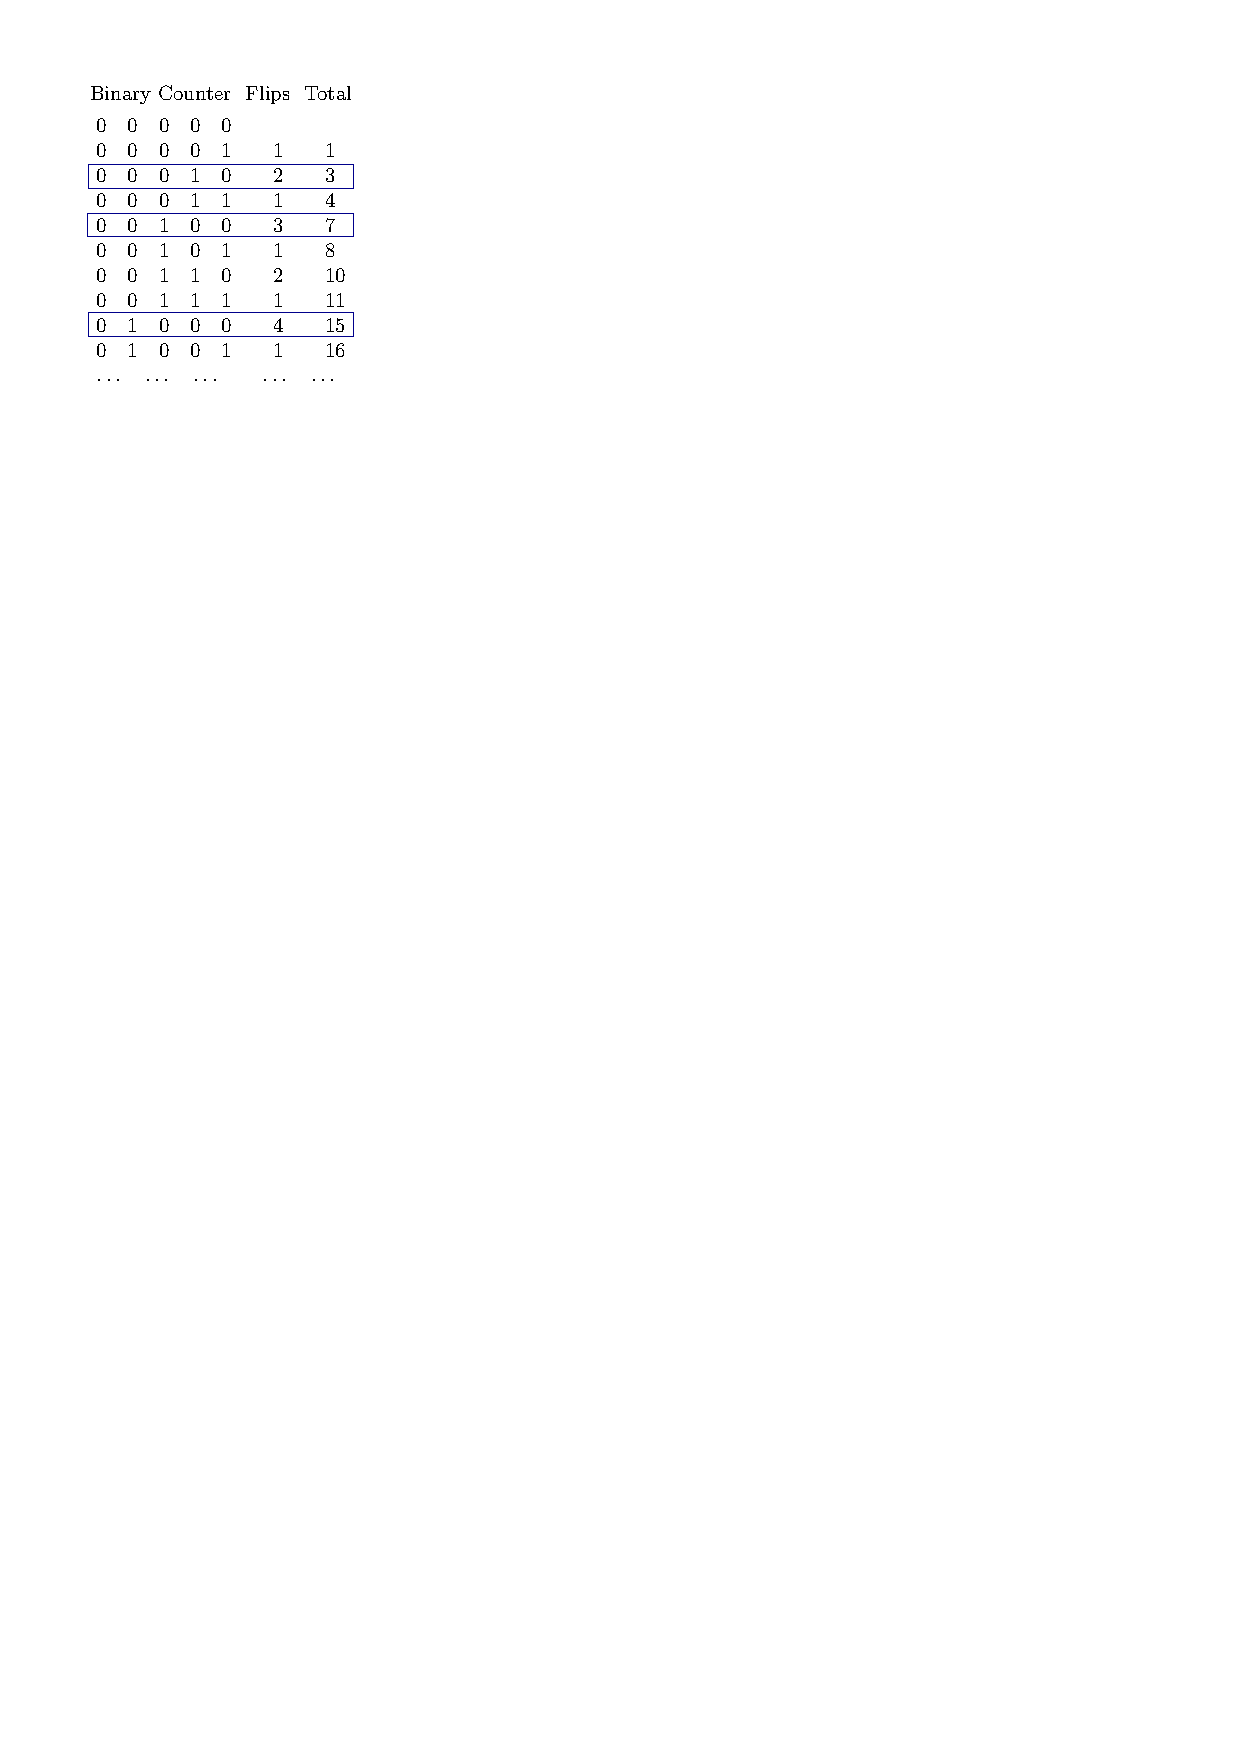
\includegraphics[scale=1]{figures/aggregate.pdf}
\caption{The process for Binary Counter operation.  The highlighted rows are those with  the most flipped bits. Total operations up to $i$th flipped bit is $2^i-1$.}
\label{fig:aggregate}
\end{figure}

As it can be seen, the total number of flips at steps where we have the most flips is equal to $2^i-1$. This gives some insight into the pattern, but it is still difficult to determine the amortized cost of the entire problem.

An alternative approach, that gives us a simpler way to count the amortized cost, is to look at each \emph{column} of bits and count the
total flips in that column.  Figure~\ref{fig:columns} illustrates how this approach lets us count the total operations needed to perform $n$ calls of \Call{Increment}{$A,k$}.
\begin{figure}[tbh]
\centering
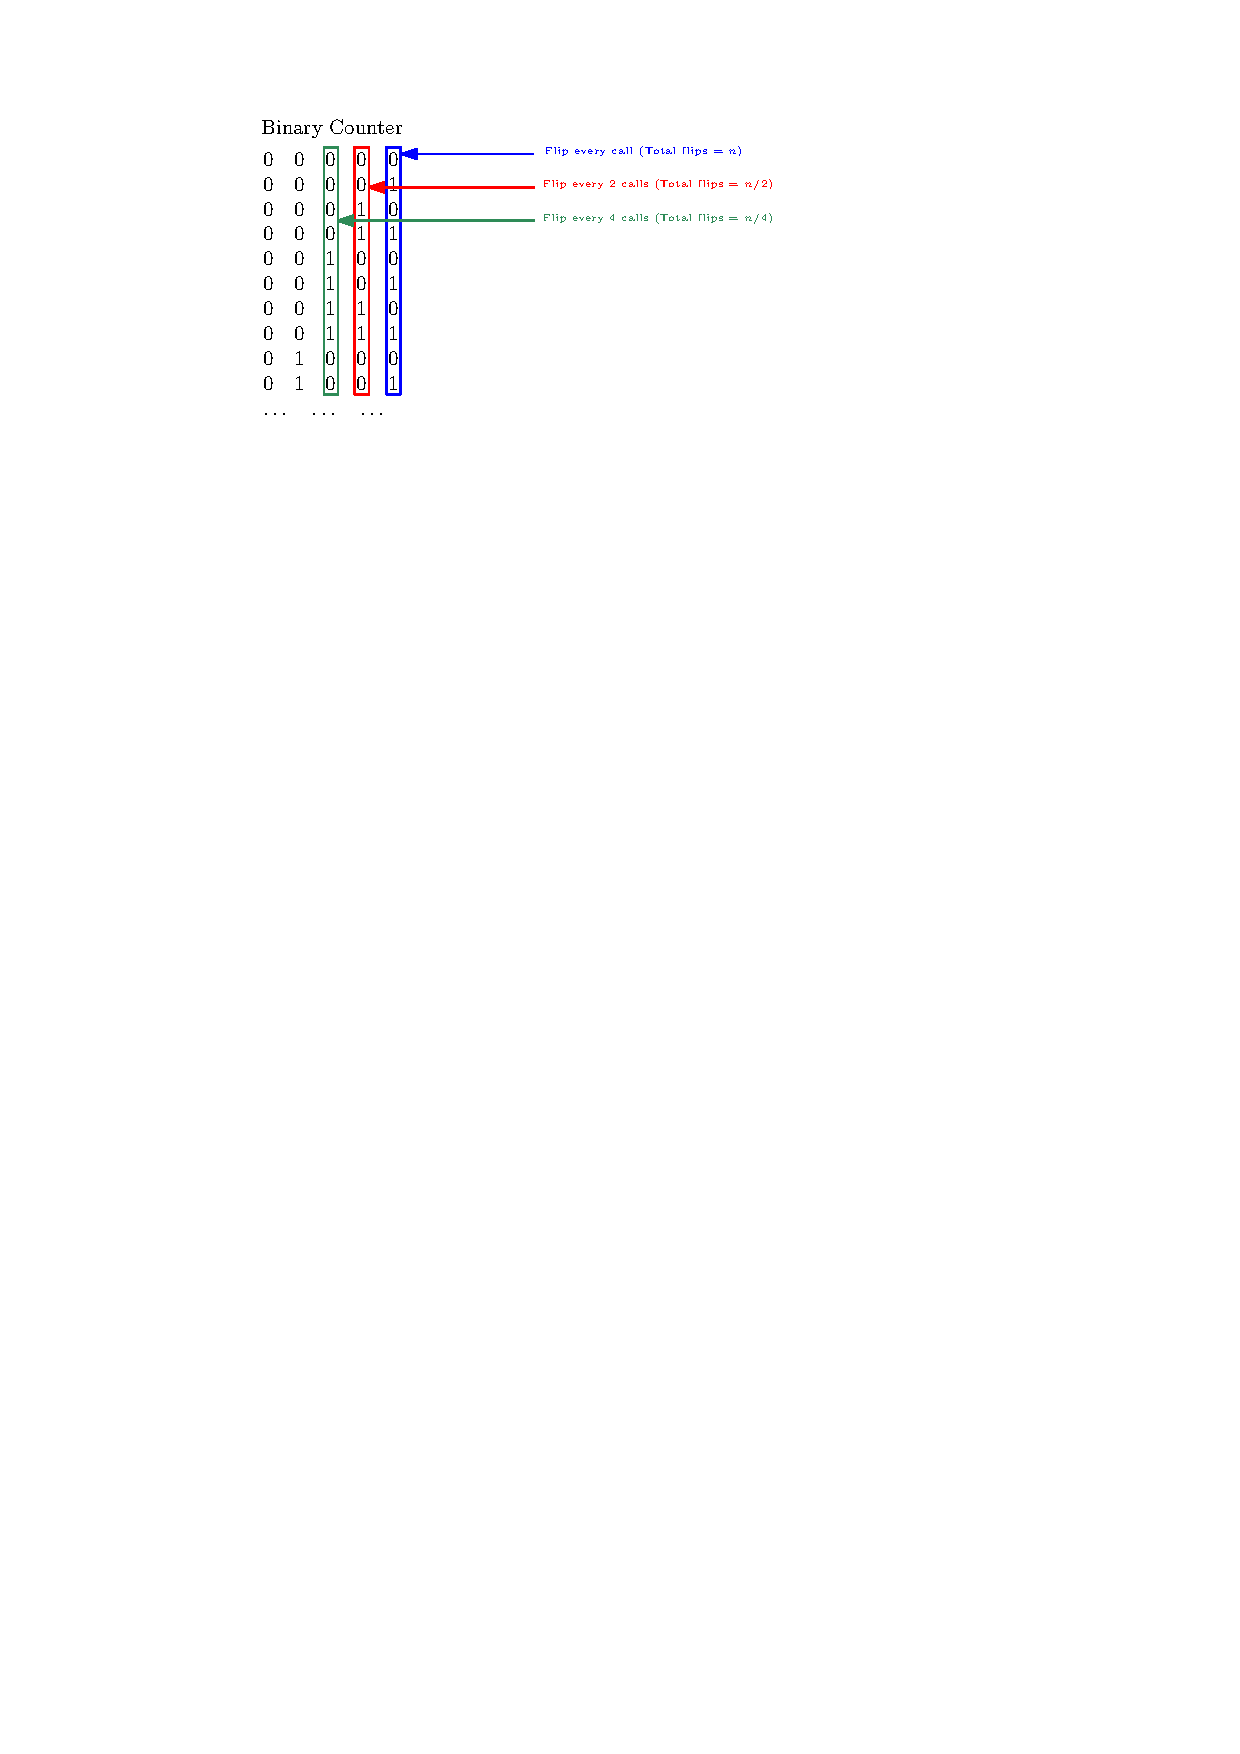
\includegraphics[scale=1]{figures/columns.pdf}
\caption{Total cost by column in aggregated method.}
\label{fig:columns}
\end{figure}

According to the figure, the first column is flipped at \emph{every} call, the second column is flipped every 2 calls, the third column is flipped every 4 calls, and so on.  This gives us the total number of flips after $n$ calls:

\begin{align*}
\text{Total \# of flips} & = n + \frac{n}{2} + \frac{n}{4} + \frac{n}{8} + \cdots + \frac{n}{2^{\log{n}}} = \sum_{i=0}^{\log{n}} \frac{n}{2^i} \\
& \leq n\sum_{i=0}^{\infty} \frac{1}{2^i} \\
& = 2n
\end{align*}

Therefore, the amortized cost $\hat{c}$ is:
\begin{align*}
\hat{c} &= \frac{\text{total \# of bit flips}}{\text{\# of calls}} \\
&= \frac{2n}{n} = 2
\end{align*}

Total amortized cost $\hat{c} = \sum_{i=1}^n \hat{c_i}$ ($\hat{c_i}$ is the amortized cost of the $i$th operation) provides us with an upper bound on the total runtime of an algorithm.  Therefore, for any $n$, total amortized cost must not
be less than the total actual cost:
\begin{align*}
\sum_{i=1}^{n}\hat{c_i} \ge \sum_{i=1}^{n} c_i
\end{align*}

Where $c_i$ is the actual cost of the $i$th call.  Thus, the total cost of $n$ calls to \Call{Increment}{$A,k$} is:
\begin{align*}
\sum_{i=1}^n c_i &\le \sum_{i=1}^n \hat{c_i} = \sum_{i=1}^n 2 = 2n\\
\end{align*}
\end{exmp}

\subsection{Accounting Method}
\label{sub:accounting}
Intuitively, we can consider the accounting method as ``saving for a rainy day.''
The idea is to allocate a fixed cost $d$ for each step of the algorithm.  Low-cost
calls will accrue ``money'' to be able to pay for more expensive calls in the future.  The steps of the accounting method are as follows:

\begin{itemize}
\item Charge $\hat{c}_i = d$ dollar for the $i$th operation,
\item Subtract actual cost $c_i$ of the operation from $d$ to pay for the operation,
\item Put the remaining $(d-c_i)$ dollar in the bank as credit to pay for future operations.
\end{itemize}

For amortized cost to be a valid upper bound on the actual cost for any number of operations, we must ensure that $\sum_{i=1}^n \hat{c_i} \ge \sum_{i=1}^n c_i$ for any $n$.  Re-ordering terms leads to:
\begin{eqnarray*}
\sum_{i=1}^{n}{\hat{c_i}} - \sum_{i=1}^{n}c_i = \sum_{i=1}^n \left(\hat{c}_i - c_i\right) \ge 0, \hspace{0.25cm} \forall n \in \mathbb{N}.
\end{eqnarray*}

In other words, the amount in the account must never drop below 0, during any step of the algorithm.  As long as this condition holds, we know that our amortized cost of $\hat{c_i}$ per operation is a valid amortized cost. 

Let's look at the example of the binary counter problem. 
We first set our cost estimate $\hat{c}_i = d = 2$ \$. Figure~\ref{fig:accounting}
illustrates how we save on low-cost operations and spend the savings on more costly ones.  In this example, we see that every time we
flip a bit from `0' to `1', the actual cost is $1$ \$, but we allocated $2$ dollar coins which means we save extra dollar as credit in the account.  We place this extra coin on the bit that has just been flipped from `0' to '1'. In the future, we will use the coins saved on `1' bits, to flip them to `0' and newly charged coins to flip `0' bits to `1'. Thus, we will never spend more coins than our savings. Figure~\ref{fig:accounting} shows how our saving is spent during the steps where we face multiple flips. 
\begin{figure}[tbh]
\centering
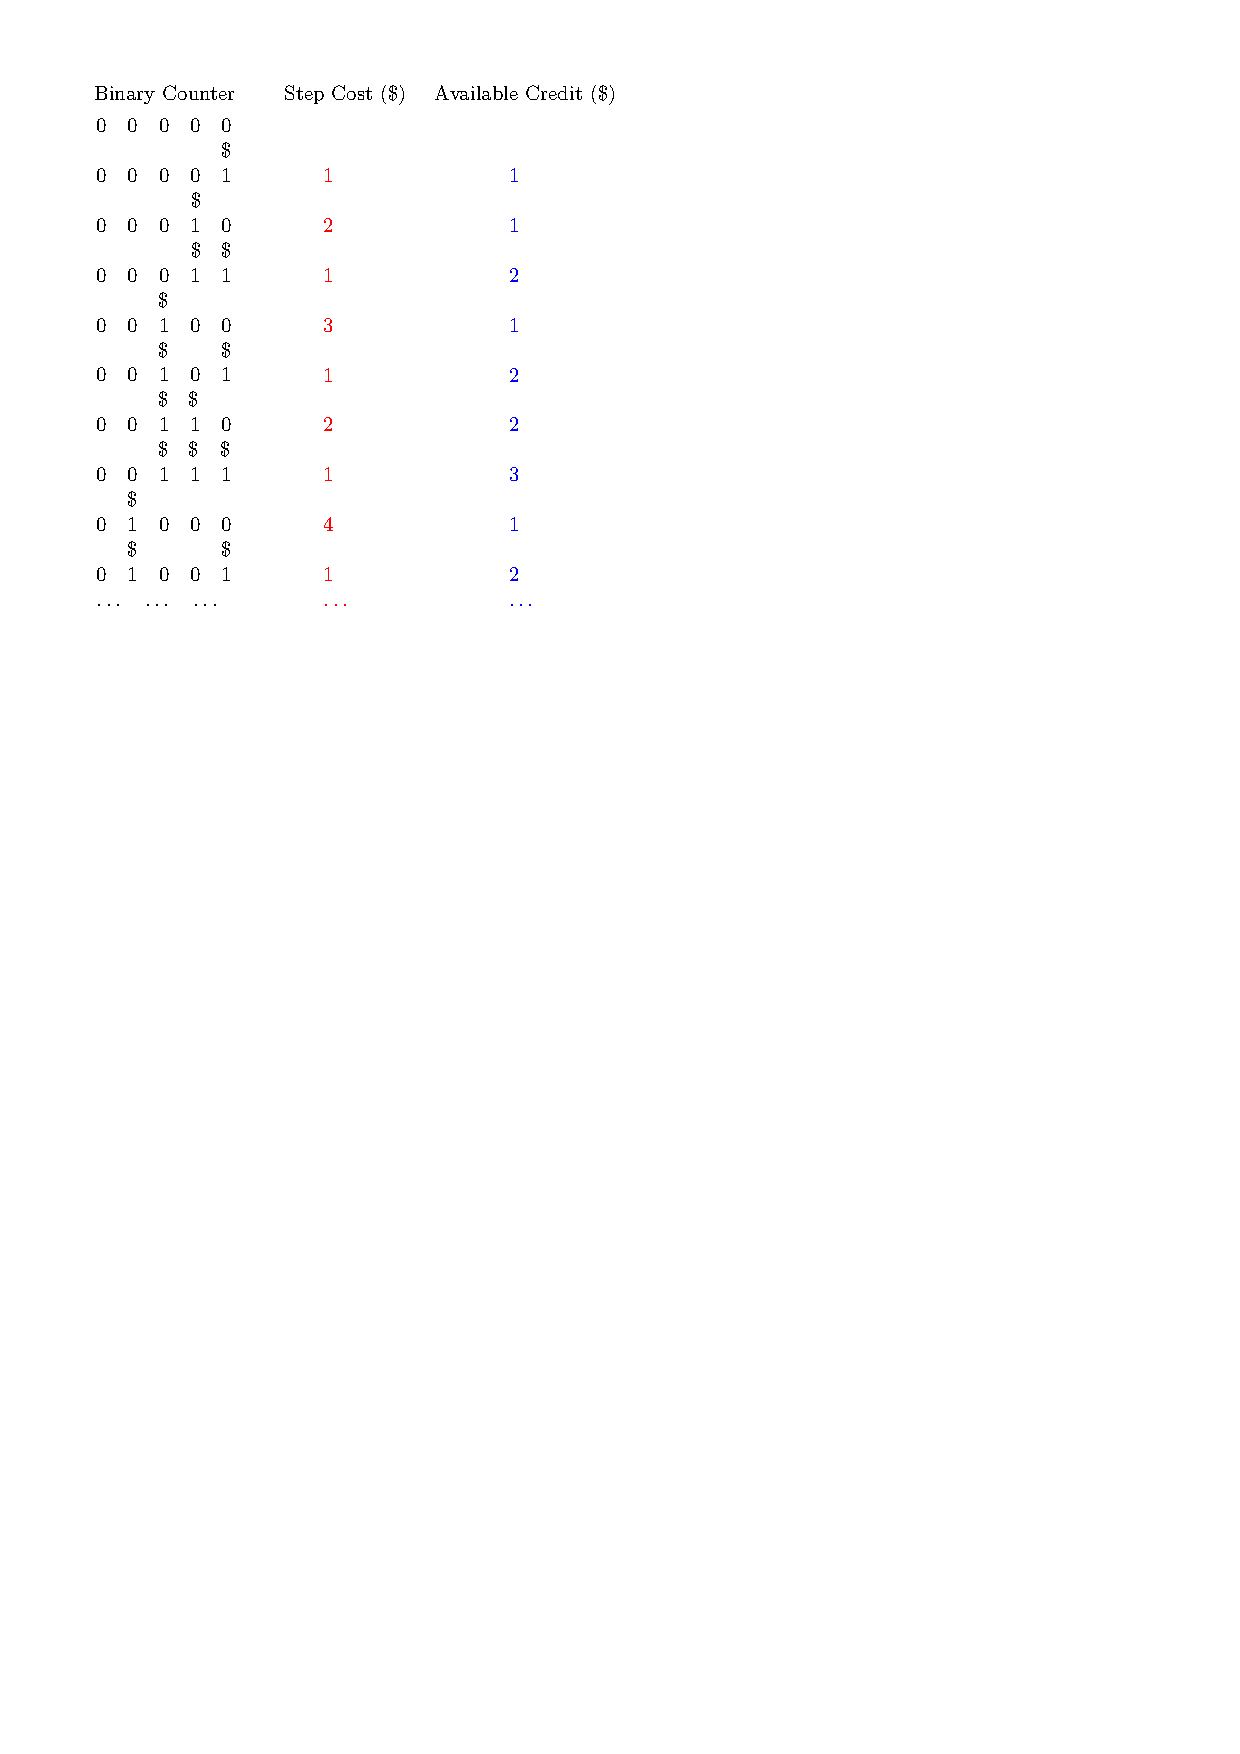
\includegraphics[scale=1]{figures/accounting.pdf}
\caption{Using Accounting method to perform amortized analysis on binary counter problem.}
\label{fig:accounting}
\end{figure}

\subsection{Dynamic Array Problem}
% \begin{myindentpar}{1cm}
% \textbf{Dynamic Array Problem}: 
Dynamic arrays are just like normal arrays but the capacity of the array is doubled every time array hits the full capacity. The cost of \Call{Append}{} operation in dynamic array is 1 when array has empty spaces but insertion operation includes cost of copying old array plus cost of inserting new item to the array when spaces are fully occupied. Dynamic arrays are a common data structure available in many programming languages.\\

\begin{algorithm}
\caption{\Call{Append}{$x,A$}}
\label{alg:dynamic_append}
\begin{algorithmic}[1]
\State Let $i = \text{ number of items in }A$
\If{$|A|=i$}
  \State $B = \text{new Array of size } 2\cdot i$
  \State $\Call{Copy}{A, B}$
  \State $A \leftarrow B$
\EndIf
\State $A[i] = x$
\State $i = i+1$
\end{algorithmic}
\end{algorithm}

The pseudocode for inserting a value into a dynamic array is shown in Algorithm: \ref{alg:dynamic_append}.
In the worst case, appending $x$ to a dynamic array using above algorithm requires copying $n$ elements. If we repeat the same operation $n$ times, it will cost us $O(n^2)$ operations. But many of \Call{Append}{} function calls won't have to copy the elements. Most of the operations will only take 1 operation(just append). Hence we can use amortized analysis to show that the amortized cost of a single append is $O(1)$.

% \end{myindentpar}

\begin{exmp}
Find the amortized cost of appending a value to a dynamic array and use the result to find appropriate cost for accounting method.\\

\textbf{Solution:}

\textbf{Aggregate Analysis:}
Using aggregate analysis, we can look at the cost of each step in Figure~\ref{fig:dynamic}.  

\begin{figure}[tbh]
\centering
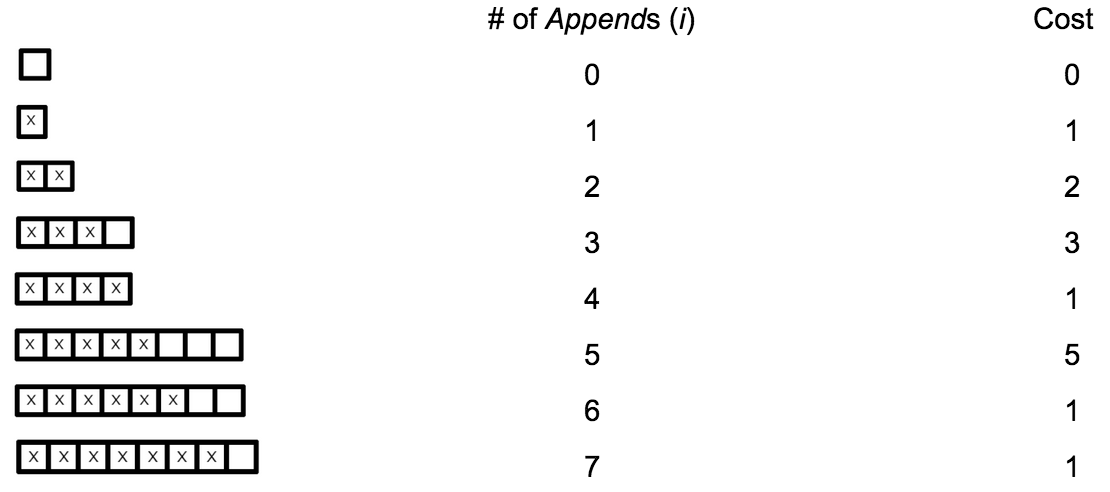
\includegraphics[scale=0.5]{figures/dynamic}
\caption{The status of the dynamic array as we insert elements into it.}
\label{fig:dynamic}
\end{figure}

As illustrated in Figure~\ref{fig:dynamic}, the cost of inserting $i$th element into the dynamic array is:

\begin{eqnarray*}
c_i = \begin{cases}
  i, & \text{if $i-1=2^k$}. \\
  1, & \text{otherwise}.
\end{cases}
\end{eqnarray*}

Now, to find the overall cost of the operation over $n$th iterations, we can sum these two terms into separate summations.

\begin{align*}
\sum_{i=1}^n c_i &= \sum_{k=0}^{\log{n}} 2^k + \sum_{i=1}^{n} 1 \\
&= 2\cdot2^{\log{n}} - 1 + n \\
&= 3n - 1
\end{align*}

This gives us an amortized cost of each call $\hat{c}_i$ = $\frac{3n-1}{n} \le 3 = O(1)$

\textbf{Accounting Method:}
Let us assume, we will charge $d$ dollars for each append to the dynamic array. We only need $\$1$ for append, so we can save $\$(d-1)$ to pay for extending and copying the value in future. We will keep track of our saved money by associating it with the newly inserted element. Each newly inserted element(which has never been copied) will have $\$(d-1)$ with them.\\

By the time we have to resize the array of size $k$, we'll have half of the elements in the array that have never been copied, so they will have $\$(d-1)$ with them. Remaining half of the elements were copied earlier i.e. they have exhausted their savings so we will use the $\$(d-1)$ (saving from new uncopied ones) to copy remaining half of the elements(those were copied in past). So we will need:

\begin{eqnarray*}
(d-1) \times \frac{k}{2} \ge k \\
d \ge 3
\end{eqnarray*}

Thus, we can charge $\hat{c}_i = 3 = O(1)$ coins for each insertion and we will never spend more than our savings during expansion of the array.

\begin{figure}[tbh]
\centering
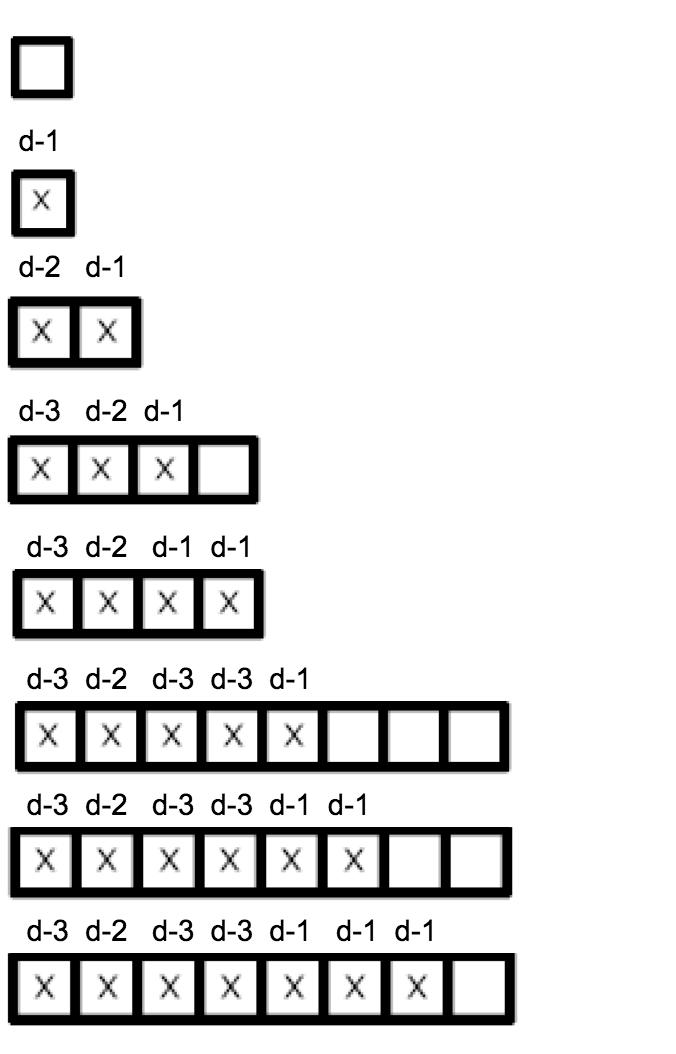
\includegraphics[scale=0.5]{figures/dynamicaccounting}
\caption{The coins accumulation account for the dynamic array insertion problem.}
\label{fig:dynamicaccounting}
\end{figure}
\end{exmp}



\subsection{Potential Method}
\label{sub:potential}

The potential method is similar to a physics outlook and looks at the ``potential'' of the entire data structure as a single value.  
We define $\Phi(D_i)$ as a function that maps a data structure $D_i$ (after the $i$th call) to a real number.
\begin{align*}
\Phi(D_i) : D_i \rightarrow \mathbb{R}&\\
\text{where } & \text{$D_i$ is the data structure after the $i$th operation}\\
&\Phi_i \text{ is potential of the data structure after the $i$th operation.}
\end{align*}

Using this potential function, $\Phi_i$, we define the amortized cost as:

\begin{eqnarray*}
\hat{c_i} = c_i + \Delta \Phi_i = c_i + (\Phi(D_i) - \Phi(D_{i-1}))
\end{eqnarray*}

Now, we can find total amortized cost for $n$ operations as:

\begin{align*}
\sum_{i=1}^{n}\hat{c_i} &= \sum_{i=1}^{n}c_i + \sum_{i=1}^{n}\Delta\Phi_i \\
&= \sum_{i=1}^{n}c_i + \sum_{i=1}^{n}(\Phi(D_i) - \Phi(D_{i-1})) \\
&= \sum_{i=1}^{n}c_i + \Phi(D_n) - \Phi(D_0)
\end{align*}

Therefore, as long as we show that our choice of the potenital function $\Phi$ results in non-negative $\Phi(D_n) - \Phi(D_0)$ for every $n$, $\hat{c}_i$ is a valid amortized cost of $i$-th operation. Furthermore, if we choose the potential function $\Phi$ such that the initial potential $\Phi(D_0)=0$, we only need to show that $\Phi(D_i)$ is non-negative, for every $i$.


\textbf{Binary Counter Problem:} To analyze the binary counter problem using the potential method, we define $\Phi$ as:

\begin{eqnarray*}
\Phi(D_i) = \text{number of 1's in the binary counter}
\end{eqnarray*}

That means, $\Phi(D_0) = \text{number of 1's in $D_0$} = 0$ and $\Phi(D_i) \ge 0$ for any $i$. \\

Now, we have \\
$\hat{c}_i = c_i + \Delta \Phi_i$

Let's define $t_i$ be the total 1's that were flipped to 0's during the $i$th call to \Call{Increment}{}.
We see that $t_i$ is the number of consecutive least significant bits that were 1's and were flipped to 0's. 
\begin{figure}[tbh]
\centering
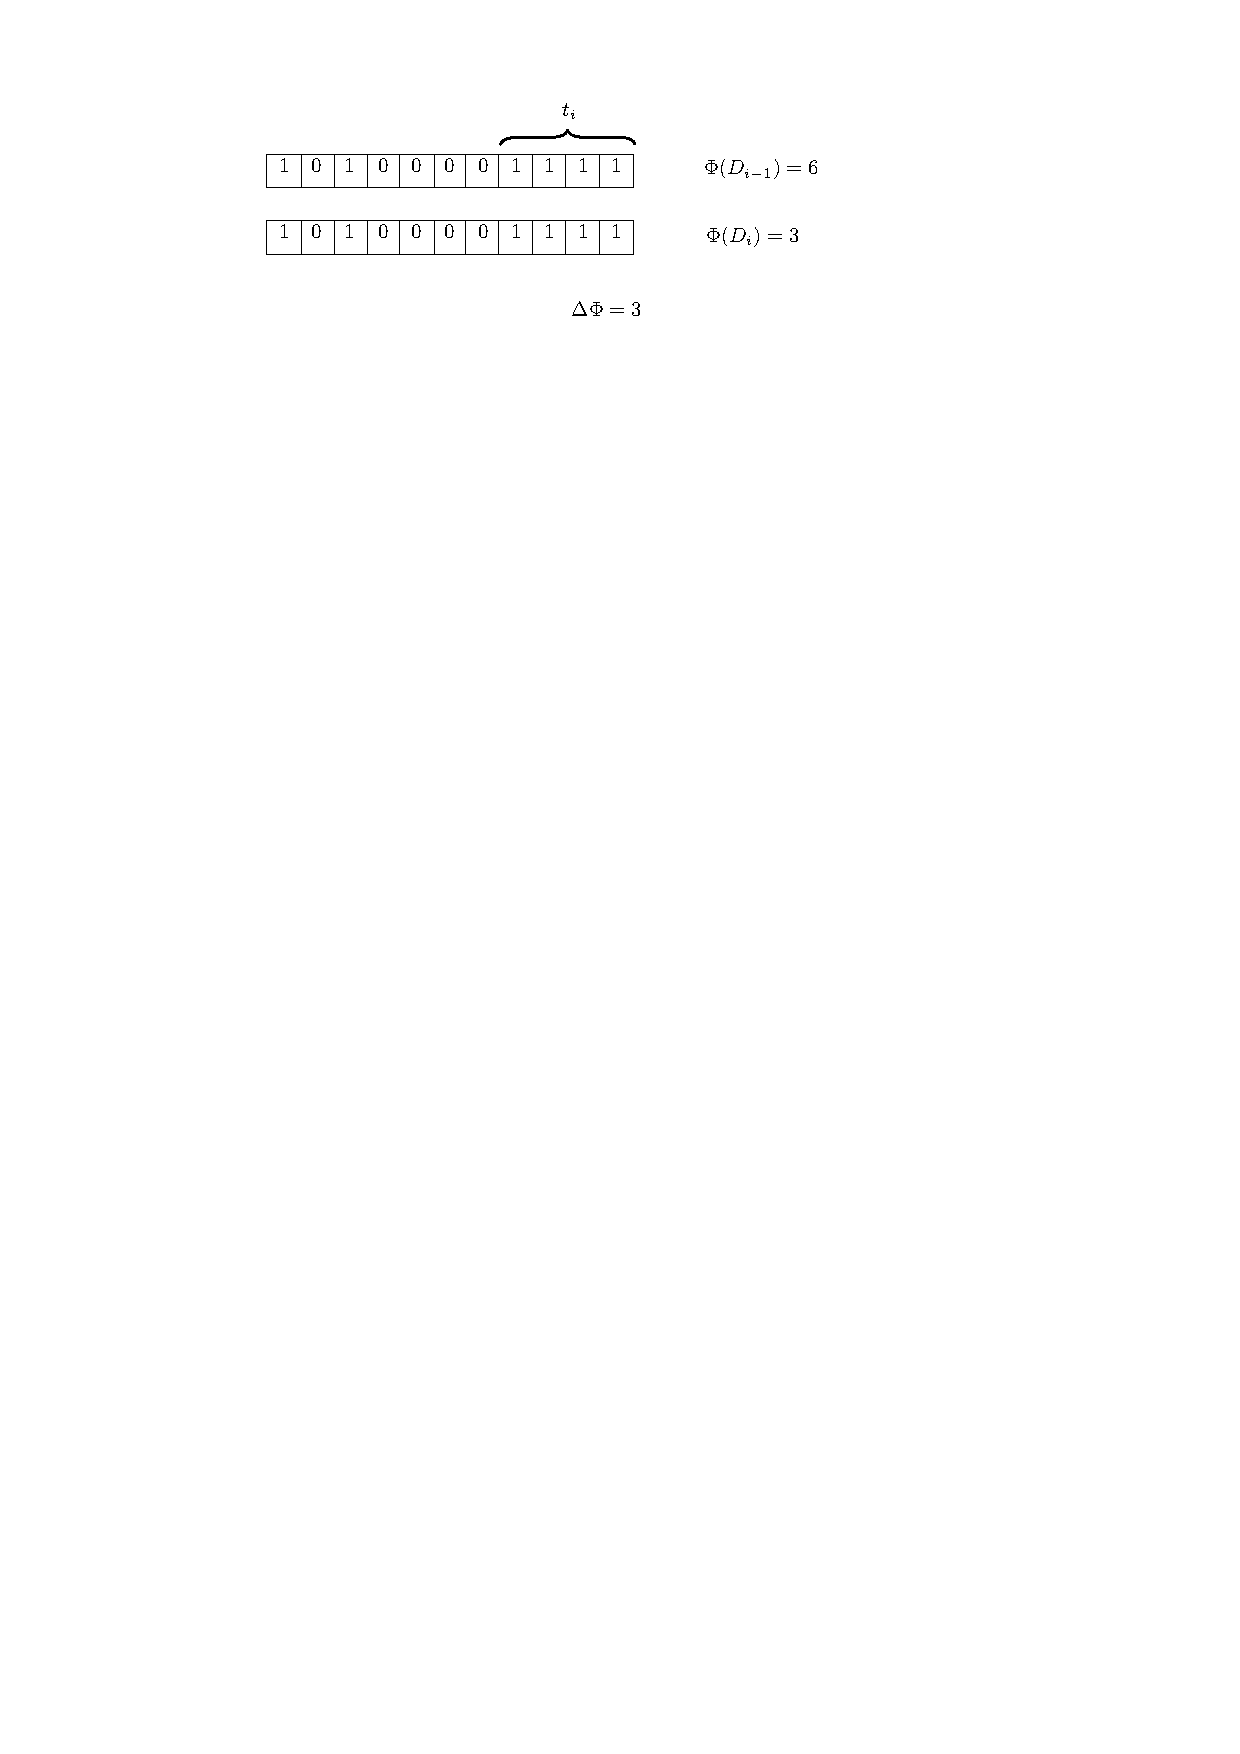
\includegraphics[scale=1]{figures/potential.pdf}
\caption{Example of the $\Phi$ potential value for the binary counter problem}
\label{fig:potential}
\end{figure}

Thus, the actual cost of the $i$-th call is $c_i = t_i+1$ ($+1$ for fliping 0 to 1).

Also total number of 1's in the binary counter after $i$th increment is given by:

\begin{align*}
\Phi(D_i) &= \text{total number of 1's in $D_{i-1} - $flipped bits} \\
          &= (\Phi(D_{i-1}) - t_i + 1)
\end{align*}

The change in the potential is:
\begin{eqnarray*}
\Delta \Phi_i = (\Phi(D_{i-1}) - t_i+1) - \Phi(D_{i-1}) = 1-t_i 
\end{eqnarray*}

Then the amortized cost of the $i$-th operation is:

\begin{eqnarray*}
\hat{c_i} &= c_i+\Delta\Phi_i = (t_i+1) + (1-t_i) = 2
\end{eqnarray*}

Thus the amortized cost for increment is $\hat{c_i} = 2 = O(1)$.





\end{document}
